% 11. Стадия 1a
\begin{frame}{Стадия 1a · Извлечение признаков}
\framesubtitle{Приведение потоков к фиксированной длине и дискретным токенам}
\vspace{1mm}
\begin{columns}[T,onlytextwidth]
\column{0.49\textwidth}
  \vspace{3mm}
  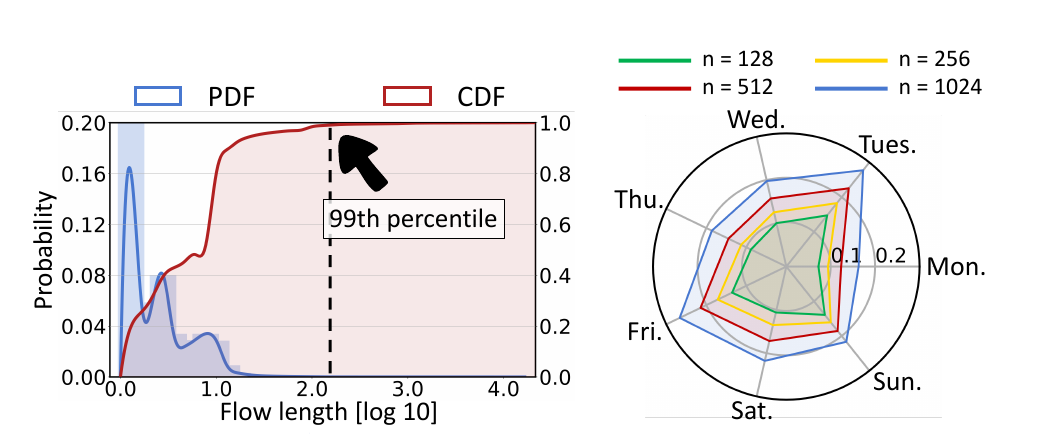
\includegraphics[width=\linewidth]{fig3.png}\par\vspace{3mm}
  \figcap{Длины потоков — «тяжёлый хвост»: берём 99-й перцентиль $\rightarrow$ $n = 512$}
\column{0.48\textwidth}
\begin{card}[height=5.8cm]\scriptsize
  \iconitem{steel}{ic_random_w.png}{\hl{Padding коротких}\ \ $m \le n$: добиваем спец-токенами [PAD]}\vspace{3.5mm}
  \iconitem{steel}{ic_layers_w.png}{\hl{Chunking длинных}\ \ $m > n$: режем на перекрывающиеся сегменты}\vspace{3.5mm}
  \iconitem{steel}{ic_code_w.png}{\hl{Токенизация}\ \ IPD $\rightarrow$ лог-интервалы; размер пакета $\rightarrow$ значение (лимит MTU, [UNK])}\vspace{3.5mm}
  \iconitem{steel}{ic_puzzle_w.png}{\hl{Эмбеддинги}\ \ токен + позиция (синусоида, сдвиг для сегментов)}
\end{card}
\end{columns}
\end{frame}
